%%%%%%%%%%%%%%%%%%%%%%%%%%%%%%%%%%%%%%%%%%%%%%
%
%		My Thesis
%
%		EDOC Template
%		2011
%
%%%%%%%%%%%%%%%%%%%%%%%%%%%%%%%%%%%%%%%%%%%%%%


%%%%%%%%%%%%%%%%%%%%%%%%%%%%%%%%%%%%%%%%%%%%%%
%
%		Thesis Settings
%
%		EDOC Template
%		2011
%
%%%%%%%%%%%%%%%%%%%%%%%%%%%%%%%%%%%%%%%%%%%%%%
\documentclass[a4paper,11pt]{book}

\usepackage[T1]{fontenc}
\usepackage[utf8]{inputenc}
% % Uncomment for bibliography
% % Bibliography using Biblatex
%\usepackage{doi}
%\usepackage[autostyle]{csquotes}
% \usepackage[
%     backend=biber,
%     style=authoryear,
%     natbib=true,
%     firstinits=true,
%     sortlocale=en_US,
%     url=false,
%     doi=true,
%     eprint=false,
%     isbn=false
% ]{biblatex}
%\addbibresource{tail/bibliography.bib}
% % OR Bibliography management for Bibtex
% Load natbib before babel
\usepackage[round]{natbib}


\usepackage[french,german,english]{babel}


%%%%%%%%%%%%%%%%%%%%%%%%%%%%%%%%%%%%%%%%%%%%%%%
%% EDOC THESIS TEMPLATE: Variant 1.0 -> Latin modern, large text width&height
%%%%%%%%%%%%%%%%%%%%%%%%%%%%%%%%%%%%%%%%%%%%%%%
\usepackage{lmodern} % use this to fix blurry typewriter text font
%\usepackage[a4paper,top=22mm,bottom=28mm,inner=35mm,outer=25mm]{geometry}
%%%%%%%%%%%%%%%%%%%%%%%%%%%%%%%%%%%%%%%%%%%%%%%

%%%%%%%%%%%%%%%%%%%%%%%%%%%%%%%%%%%%%%%%%%%%%%
% EDOC THESIS TEMPLATE: Variant 2.0 -> Utopia, Gabarrit A (lighter pages)
%%%%%%%%%%%%%%%%%%%%%%%%%%%%%%%%%%%%%%%%%%%%%%
\usepackage{fourier} % Utopia font-typesetting including mathematical formula compatible with newer TeX-Distributions (>2010)
%\usepackage{utopia} % on older systems -> use this package instead of fourier in combination with mathdesign for better looking results
%\usepackage[adobe-utopia]{mathdesign}
\setlength{\textwidth}{146.8mm} % = 210mm - 37mm - 26.2mm
\setlength{\oddsidemargin}{11.6mm} % 37mm - 1in (from hoffset)
\setlength{\evensidemargin}{0.8mm} % = 26.2mm - 1in (from hoffset)
\setlength{\topmargin}{-2.2mm} % = 0mm -1in + 23.2mm
\setlength{\textheight}{221.9mm} % = 297mm -29.5mm -31.6mm - 14mm (12 to accomodate footline with pagenumber)
\setlength{\headheight}{14pt}
%%%%%%%%%%%%%%%%%%%%%%%%%%%%%%%%%%%%%%%%%%%%%%


\usepackage{setspace} % increase interline spacing slightly
\setstretch{1.1}

\makeatletter
\setlength{\@fptop}{0pt}  % for aligning all floating figures/tables etc... to the top margin
\makeatother


\usepackage{graphicx}
\usepackage[table]{xcolor}
\graphicspath{{images/}}

\usepackage{subfig}
\usepackage{booktabs}
\usepackage{lipsum}
\usepackage{microtype}
\usepackage{url}

\usepackage{fancyhdr}
\renewcommand{\sectionmark}[1]{\markright{\thesection\ #1}}
\pagestyle{fancy}
	\fancyhf{}
	\renewcommand{\headrulewidth}{0.4pt}
	\renewcommand{\footrulewidth}{0pt}
	\fancyhead[OR]{\bfseries \nouppercase{\rightmark}}
	\fancyhead[EL]{\bfseries \nouppercase{\leftmark}}
	\fancyfoot[EL,OR]{\thepage}
\fancypagestyle{plain}{
	\fancyhf{}
	\renewcommand{\headrulewidth}{0pt}
	\renewcommand{\footrulewidth}{0pt}
	\fancyfoot[EL,OR]{\thepage}}
\fancypagestyle{addpagenumbersforpdfimports}{
	\fancyhead{}
	\renewcommand{\headrulewidth}{0pt}
	\fancyfoot{}
	\fancyfoot[RO,LE]{\thepage}
}

\usepackage{listings}
\lstset{language=[LaTeX]Tex,tabsize=4, basicstyle=\scriptsize\ttfamily, showstringspaces=false, numbers=left, numberstyle=\tiny, numbersep=10pt, breaklines=true, breakautoindent=true, breakindent=10pt}

\usepackage{hyperref}
\hypersetup{pdfborder={0 0 0},
	colorlinks=true,
	linkcolor=black,
	citecolor=black,
	urlcolor=black}
\urlstyle{same}
\ifpdf
\usepackage[final]{pdfpages}
\else
\usepackage{calc}
\usepackage{breakurl}
\usepackage[nlwarning=false]{hypdvips}
\usepackage{backref}
\renewcommand*{\backref}[1]{}
\fi
\usepackage{bookmark}

\makeatletter
\renewcommand\@pnumwidth{20pt}
\makeatother

\makeatletter
\def\cleardoublepage{\clearpage\if@twoside \ifodd\c@page\else
    \hbox{}
    \thispagestyle{empty}
    \newpage
    \if@twocolumn\hbox{}\newpage\fi\fi\fi}
\makeatother \clearpage{\pagestyle{plain}\cleardoublepage}


%%%%% CHAPTER HEADER %%%%
\usepackage{color}
\usepackage{tikz}
\usepackage[explicit]{titlesec}
\newcommand*\chapterlabel{}
%\renewcommand{\thechapter}{\Roman{chapter}}
\titleformat{\chapter}[display]  % type (section,chapter,etc...) to vary,  shape (eg display-type)
	{\normalfont\bfseries\Huge} % format of the chapter
	{\gdef\chapterlabel{\thechapter\ }}     % the label
 	{0pt} % separation between label and chapter-title
 	  {\begin{tikzpicture}[remember picture,overlay]
    \node[yshift=-8cm] at (current page.north west)
      {\begin{tikzpicture}[remember picture, overlay]
        \draw[fill=black] (0,0) rectangle(35.5mm,15mm);
        \node[anchor=north east,yshift=-7.2cm,xshift=34mm,minimum height=30mm,inner sep=0mm] at (current page.north west)
        {\parbox[top][30mm][t]{15mm}{\raggedleft \rule{0cm}{0.6cm}\color{white}\chapterlabel}};  %the empty rule is just to get better base-line alignment
        \node[anchor=north west,yshift=-7.2cm,xshift=37mm,text width=\textwidth,minimum height=30mm,inner sep=0mm] at (current page.north west)
              {\parbox[top][30mm][t]{\textwidth}{\rule{0cm}{0.6cm}\color{black}#1}};
       \end{tikzpicture}
      };
   \end{tikzpicture}
   \gdef\chapterlabel{}
  } % code before the title body
\titlespacing*{name=\chapter,numberless}{-3.7cm}{83.2pt-\parskip}{-3.2pt+\parskip}
\titlespacing*{\chapter}{-3.7cm}{50pt-\parskip-\parskip}{30pt+\parskip+\parskip}
\titlespacing*{\section}{0pt}{13.2pt}{1em-\parskip}  % 13.2pt is line spacing for a text with 11pt font size
\titlespacing*{\subsection}{0pt}{13.2pt}{1em-\parskip}
\titlespacing*{\subsubsection}{0pt}{13.2pt}{1em-\parskip}
\titlespacing*{\paragraph}{0pt}{13.2pt}{1em-\parskip}

\newcounter{myparts}
\newcommand*\partlabel{}
\titleformat{\part}[display]  % type (section,chapter,etc...) to vary,  shape (eg display-type)
	{\normalfont\bfseries\Huge} % format of the part
	{\gdef\partlabel{\thepart\ }}     % the label
 	{0pt} % separation between label and part-title
 	  {\ifpdf\setlength{\unitlength}{20mm}\else\setlength{\unitlength}{0mm}\fi
	  \addtocounter{myparts}{1}
	  \begin{tikzpicture}[remember picture,overlay]
    \node[anchor=north west,xshift=-65mm,yshift=-6.9cm-\value{myparts}*20mm] at (current page.north east) % for unknown reasons: 3mm missing -> 65 instead of 62
      {\begin{tikzpicture}[remember picture, overlay]
        \draw[fill=black] (0,0) rectangle(62mm,20mm);   % -\value{myparts}\unitlength
        \node[anchor=north west,yshift=-6.1cm-\value{myparts}*\unitlength,xshift=-60.5mm,minimum height=30mm,inner sep=0mm] at (current page.north east)
        {\parbox[top][30mm][t]{55mm}{\raggedright \color{white}Part \partlabel \rule{0cm}{0.6cm}}};  %the empty rule is just to get better base-line alignment
        \node[anchor=north east,yshift=-6.1cm-\value{myparts}*\unitlength,xshift=-63.5mm,text width=\textwidth,minimum height=30mm,inner sep=0mm] at (current page.north east)
              {\parbox[top][30mm][t]{\textwidth}{\raggedleft \rule{0cm}{0.6cm}\color{black}#1}};
       \end{tikzpicture}
      };
   \end{tikzpicture}
   \gdef\partlabel{}
  } % code before the title body
\titlespacing*{\part}{11.06cm}{26.4pt-\parskip-\parskip}{0pt}

\usepackage{amsmath}
\usepackage{amsfonts}
\usepackage{amssymb}
\usepackage{mathtools}
% Fix the problem with delimiter size caused by fourier and amsmath packages.
\makeatletter
\def\resetMathstrut@{%
  \setbox\z@\hbox{%
    \mathchardef\@tempa\mathcode`\(\relax
      \def\@tempb##1"##2##3{\the\textfont"##3\char"}%
      \expandafter\@tempb\meaning\@tempa \relax
  }%
  \ht\Mathstrutbox@1.2\ht\z@ \dp\Mathstrutbox@1.2\dp\z@
}
\makeatother

% !TEX root = ../sethomas_thesis_main.tex
%%%%%%%%%%%%%%%%%%%%%%%%%%%%%%%%%%%%%%%%%%%%%%
%
%		Thesis Settings
%		Custom settings
%
%		2011
%
%%%%%%%%%%%%%%%%%%%%%%%%%%%%%%%%%%%%%%%%%%%%%%

% %
% %   Use this file for your own custom packages, command-definitions, etc...
% %
% %
% % Packages for references - cleverref must be last
% \usepackage{nameref}
% \usepackage{hyperref}
\usepackage{cleveref}
\usepackage{multicol}
\usepackage{multirow}
\usepackage{makecell}
\usepackage{overpic} % picture in picture
\usepackage{pict2e} % For the polygon function in overpic
\usepackage{siunitx}
\usepackage{tabu}
\usepackage{array}
\newcolumntype{P}[1]{>{\centering\arraybackslash}p{#1}} % New centered column with variable width
\usepackage{framed}
% \usepackage{tikz-dimline}
\usepackage{caption}
\usepackage{subcaption}
\usepackage{rotating}   % For sideways table
\usepackage{lscape}
\usepackage{afterpage}
\usepackage{standalone} % For seperature figure tex files

% \usepackage[shortlabels]{enumitem}
% % Reduce spacing in bibliography
% \setlength{\bibsep}{0pt plus 0.3ex}
% % Allow equations to break between pages
% \allowdisplaybreaks
% % Penalty for widow and orphan
% \widowpenalty=9999
% \clubpenalty=9999
% %Penalty for relation and binary operation breaks in equations
% \relpenalty=9999
% \binoppenalty=9999

%%%%%%%%%% FLOW CHART %%%%%%%%%%%%%
\usetikzlibrary{calc,trees,positioning,arrows,chains,shapes.geometric,%
    decorations.pathreplacing,decorations.pathmorphing,decorations.markings,shapes,%
    matrix,shapes.symbols,positioning,angles,quotes,patterns}

\tikzstyle{textbox} = [rectangle, rounded corners, minimum width=3cm, minimum height=1cm,text centered, text width=3cm, draw=black, fill=white]
\tikzstyle{arrow} = [thick,->,>=stealth]

%%%%%%%%%% CIRCUIT TIKZ %%%%%%%%%%%
\usetikzlibrary{spy,shapes.multipart,babel}
\usepackage[siunitx,europeanresistors,EFvoltages]{circuitikz} % To have the european convention for the drawing of electrical components. Also to have the current and voltage arrows going from high to low potential
\ctikzset{voltage/bump b=18pt,voltage/european label distance=15pt,voltage/distance from node=.1}

%%%%%%%%%% DIAGRAMS %%%%%%%%%%%%%
%See https://tex.stackexchange.com/a/29367/1952
\makeatletter
\tikzset{% customization of pattern
        hatch distance/.store in=\hatchdistance,
        hatch distance=5pt,
        hatch thickness/.store in=\hatchthickness,
        hatch thickness=5pt
        }
\pgfdeclarepatternformonly[\hatchdistance,\hatchthickness]{north east hatch}% name
    {\pgfqpoint{-1pt}{-1pt}}% below left
    {\pgfqpoint{\hatchdistance}{\hatchdistance}}% above right
    {\pgfpoint{\hatchdistance-1pt}{\hatchdistance-1pt}}%
    {
        \pgfsetcolor{\tikz@pattern@color}
        \pgfsetlinewidth{\hatchthickness}
        \pgfpathmoveto{\pgfqpoint{0pt}{0pt}}
        \pgfpathlineto{\pgfqpoint{\hatchdistance}{\hatchdistance}}
        \pgfusepath{stroke}
    }
\makeatother



%%%%%%%%%%%%%%%%%%%%%%%%%%%%%%%%%%%%%%%%%%%%%%
%
%       Custom Commands
%
%%%%%%%%%%%%%%%%%%%%%%%%%%%%%%%%%%%%%%%%%%%%%%
\newcommand{\todocite}{{\color{red}cite}}
% To circle some numbers (require the tikz package) :  \circled{<number>}
\newcommand*\bigcircled[1]{\tikz[baseline=(char.base)]{
            \node[shape=circle,draw,inner sep=2pt] (char) {#1};}}
\DeclareRobustCommand \circled[1]{\tikz[baseline=(char.base)]{
            \node[shape=circle,draw,inner sep=0.4pt] (char) {#1};}}


\newcommand{\degreeC}{$^{\circ}$C~}

% Thick lines for tabular
\makeatletter
\newcommand{\thickhline}{%
    \noalign {\ifnum 0=`}\fi \hrule height 1pt
    \futurelet \reserved@a \@xhline
}
\newcolumntype{"}{@{\hskip\tabcolsep\vrule width 1pt\hskip\tabcolsep}}
\makeatother

%%%%%%%%% FIGURE LEGENDS %%%%%%%%%%%%%

% Dotted line for legends
\newcommand{\dottedrule}{ \rule[2pt]{1pt}{0.5mm} \rule[2pt]{1pt}{0.5mm} \rule[2pt]{1pt}{0.5mm}}

\newcommand{\dhorline}[3][0]{%
    \tikz[baseline]{\path[decoration={markings,
      mark=between positions 0 and 1 step 2*#3
      with {\node[fill, circle, minimum width=#3, inner sep=0pt, anchor=south west] {};}},postaction={decorate}]  (0,#1+1.5pt) -- ++(#2,0);}}
\newcommand{\dvertline}[3][0]{%
    \tikz[baseline]{\path[decoration={markings,
      mark=between positions 0 and 1 step 2*#2
      with {\node[fill, circle, minimum width=#2, inner sep=0pt, anchor=south west] {};}},postaction={decorate}] (0, #1) -- ++(0,#3);}}

%%%%%%%%% ANNOTATING IMAGES %%%%%%%%%%%%%
\usepackage{tikz-imagelabels}

\imagelabelset{
   coarse grid color = red,
   fine grid color = gray,
   image label font = \sffamily\bfseries\small,
   image label distance = 2mm,
   image label back = black,
   image label text = white,
   coordinate label font = \sffamily\bfseries\small,
   coordinate label distance = 2mm,
   coordinate label back = none,
   coordinate label text = white,
   annotation font = \normalfont\small,
   arrow distance = 0mm,
   border thickness = 0.6pt,
   arrow thickness = 0.4pt,
   tip size = 1.2mm,
   outer dist = 0.1cm,
}
%%%%%%%%%%%%%%%%%%%%%%%%%%%%%%%%%%%%

% Inserts a scale bar into an image
% Optional argument 1: the colour of the bar and text
% Argument 2: an \includegraphics command
% Argument 3: the real world width of the image
% Argument 4: the length of the scale bar in pixels
% Argument 5: the length of the scale bar in mm
\newcommand{\scalebar}[5][white]{
 \begin{tikzpicture}
  \node[anchor=south west,inner sep=0] (image) { #2 };
  \begin{scope}[x={(image.south east)},y={(image.north west)}]
   \draw [#1, line width=0.4em] (0.04,1.2em) -- node[above,inner sep=0.3em, font=\normalsize] {\SI{#5}{\milli \meter}} (#5*#4/#3+0.04,1.2em);
  \end{scope}
 \end{tikzpicture}
}

%%%%%%%%%%%%%%%%%%%%%%%%%%%%%%%%%%%%%%%%%%%%%%%%%%%%%%%%%%%%%%%%%%%%%%
% LaTeX Overlay Generator - Annotated Figures v0.0.1
% Created with http://ff.cx/latex-overlay-generator/
% If this generator saves you time, consider donating 5,- EUR! :-)
%%%%%%%%%%%%%%%%%%%%%%%%%%%%%%%%%%%%%%%%%%%%%%%%%%%%%%%%%%%%%%%%%%%%%%
%\annotatedFigureBoxCustom{bottom-left}{top-right}{label}{label-position}{box-color}{label-color}{border-color}{text-color}
\newcommand*\annotatedFigureBoxCustom[8]{\draw[#5,ultra thick,rounded corners, opacity=0.8] (#1) rectangle (#2);\node at (#4) [fill=#6,ultra thick,shape=circle,draw=#7,inner sep=2pt,font=\sffamily,text=#8, opacity=0.8] {\textbf{#3}};}
%\annotatedFigureBox{bottom-left}{top-right}{label}{label-position}
\newcommand*\annotatedFigureBox[5]{\annotatedFigureBoxCustom{#1}{#2}{#3}{#4}{#5}{white}{#5}{#5}}
\newcommand*\annotatedFigureText[4]{\node[draw=none, anchor=south west, text=#2, inner sep=0, text width=#3\linewidth,font=\sffamily] at (#1){#4};}
\newenvironment {annotatedFigure}[1]{\centering\begin{tikzpicture}
\node[anchor=south west,inner sep=0] (image) at (0,0) { #1};\begin{scope}[x={(image.south east)},y={(image.north west)}]}{\end{scope}\end{tikzpicture}}

%%%%% ROUNDED CORNERS IMAGE %%%%%%
\newsavebox{\picbox}
\newcommand{\cutpic}[3]{
  \savebox{\picbox}{\includegraphics[width=#2]{#3}}
  \tikz\node [draw, rounded corners=#1, line width=4pt,
    color=white, minimum width=\wd\picbox,
    minimum height=\ht\picbox, path picture={
      \node at (path picture bounding box.center) {
        \usebox{\picbox}};
    }] {};}
%%%% GET WIDTH AND HEIGHT OF NODE %%%%%%%%
\makeatletter
% Stuff for calc compatiability.
\let\real=\pgfmath@calc@real
\let\minof=\pgfmath@calc@minof
\let\maxof=\pgfmath@calc@maxof
\let\ratio=\pgfmath@calc@ratio
\let\widthof=\pgfmath@calc@widthof
\let\heightof=\pgfmath@calc@heightof
\let\depthof=\pgfmath@calc@depthof
\makeatother
%%%%%%%%%%%%%%%%%%%%%%%%%%%%%%%%%%%%%%%%%%%%%%%%%%%%%%%%%%%%%%%%%%%%%%

%%%%%%%%%%%%%% COLORS %%%%%%%%%%%%%%%%%%%%%%%%%%%%%%%
\definecolor{myblue}{HTML}{0072BD}
\definecolor{mygreen}{HTML}{258F1B}
\definecolor{myred}{HTML}{C4000C}
\definecolor{myyellow}{HTML}{F2C335}
\definecolor{myblack}{HTML}{282C34}
\definecolor{darkgreen}{HTML}{0D330A}
\definecolor{lightgreen}{HTML}{32C326}
\definecolor{darkblue}{HTML}{09299E}
\definecolor{lightblue}{HTML}{367DD9}
\definecolor{lightgrey}{HTML}{6A6A6A}
\definecolor{darkgrey}{HTML}{1E1E1E}

\definecolor{lightcolor}{HTML}{97C8DB}
\definecolor{middlecolor}{HTML}{4090BE}
\definecolor{darkcolor}{HTML}{24498B}

%%%%%%%%%%%%%%%%%%%%%%%%%%%%%%%%%%%%%%%%%%%%%%%%%%%%%%%%%%%%%%%%%%%%%%%%%%%%%%%%
%%%%%%%%%%%%%%%%%%%%%%% VARIABLES %%%%%%%%%%%%%%%%%%%%%%%%%%%%%%%%%%%%%%%%%%%%%%
%%%%%%%%%%%%%%%%%%%%%%%%%%%%%%%%%%%%%%%%%%%%%%%%%%%%%%%%%%%%%%%%%%%%%%%%%%%%%%%%
\newcommand{\StrainRetention}{\ensuremath{\alpha_\epsilon}} % Strain
\newcommand{\Domain}{\ensuremath{\Omega}} % Design domain
\newcommand{\ObjFct}{\gamma} % Objective function
\newcommand{\IniOpt}[1]{\ensuremath{\widetilde{#1}^*}} % Optimal value of #1 when optimized alone
\newcommand{\ObjFctDec}{\gamma} % Infinideciaml evaluation of the Objective function
\newcommand{\EquFct}{h} % Equality constraint function
\newcommand{\IneqFct}{g} % Inequality constraint function
% \newcommand{\Pot}{\ensuremath{u}} % Function depending on the design variable (Usually a potential found with FEA)
\newcommand{\MIS}{\text{MIS}}  % Material Interpolation Function
\newcommand{\ArtDen}{\ensuremath{\rho}} % Artificial density
\newcommand{\FiltArtDen}{\widetilde{\ArtDen}} % Filtered Artificial Densities
\newcommand{\NbEQ}{NEC} % Number of equality constraints
\newcommand{\NbINEQ}{NIC} % Number of inequality constraints

\newcommand{\Volume}{\text{Vol}} %Volume of the resulting topology
\newcommand{\PenFac}{n} % penalization factor in SIMP model
\newcommand{\FiltRadius}{\ensuremath{r_\text{min}}} % radius of the filter (r_min usually imply a minimal lenghtscale)


\newcommand{\NSubObj}{\text{NF}} % Number of sub-objectives
\newcommand{\WeightSubObj}{\ensuremath{\alpha}}

\newcommand{\Lagran}{L}
\newcommand{\LagranParam}{\ensuremath{\lambda}}


%%%%%%%%%%%%%%%%%%%%%%%%%%%%%%%%%%%%%%%%%%%%%%%%%%%%%%%%%%%%%%%%%%%%%%%%%%%%%%%%
%%%%%%%%%%%%%%%%%%%%%% Structural %%%%%%%%%%%%%%%%%%%%%%%%%%%%%%%%%%%%%%%%%%%%%%
%%%%%%%%%%%%%%%%%%%%%%%%%%%%%%%%%%%%%%%%%%%%%%%%%%%%%%%%%%%%%%%%%%%%%%%%%%%%%%%%
\newcommand{\YoungModulus}{\text{E}} % Young modulus
\newcommand{\PoissonRatio}{\ensuremath{\nu}} % Poisson's ratio of the material $\ArtDen_\text{min}$
\newcommand{\Stiffness}{\text{k}} % stiffness coeficient
\newcommand{\Load}{\text{F}} % Load
\newcommand{\Disp}{\text{U}} % Displacements
\newcommand{\EStrain}{\text{S}} % Strain energy



%%%%%%%%%%%%%%%%%%%%%%%%%%%%%%%%%%%%%%%%%%%%%%%%%%%%%%%%%%%%%%%%%%%%%%%%%%%%%%%%
%%%%%%%%%%%%%%%%% Finite Element Analysis %%%%%%%%%%%%%%%%%%%%%%%%%%%%%%%%%%%%%%
%%%%%%%%%%%%%%%%%%%%%%%%%%%%%%%%%%%%%%%%%%%%%%%%%%%%%%%%%%%%%%%%%%%%%%%%%%%%%%%%
\newcommand{\ShapeFct}{\ensuremath{\phi}}
\newcommand{\StiffMat}{\text{K}}
\newcommand{\NDesElem}{\text{NE}}
\newcommand{\NNodes}{\text{NN}} % Number of nodes of the design elements
\newcommand{\NEROI}{\ensuremath{\text{NE}_\text{ROI}}}
\newcommand{\NROI}{\ensuremath{\text{N}_\text{ROI}}}
\newcommand{\VolumeElem}{\ensuremath{V}}
\newcommand{\LengthElem}{\ensuremath{l}}
\newcommand{\elemROI}{r}
\newcommand{\elem}{e}
\newcommand{\node}{n}
\newcommand{\elemJ}{j}


%%%%%%%%%%%%%%%%%%%%%%%%%%%%%%%%%%%%%%%%%%%%%%%%%%%%%%%%%%%%%%%%%%%%%%%%%%%%%%%%
%%%%%%%%%%%%%%%%%%%%%%%%%%%%%%%% Geometry %%%%%%%%%%%%%%%%%%%%%%%%%%%%%%%%%%%%%%
%%%%%%%%%%%%%%%%%%%%%%%%%%%%%%%%%%%%%%%%%%%%%%%%%%%%%%%%%%%%%%%%%%%%%%%%%%%%%%%%

\newcommand{\thickness}{t} % Thickness of the considered plane
\newcommand{\width}{w} % Width of the design domain
\newcommand{\height}{h} % Height of the design domain

%%%%%%%%%%%%%%%%%%%%%%%%%%%%%%%%%%%%%%%%%%%%%%%%%%%%%%%%%%%%%%%%%%%%%%%%%%%%%%%%%%
%%%%%%%%%%%%%%%%%%%%%%%%%%%% Induction heating %%%%%%%%%%%%%%%%%%%%%%%%%%%%%%%%%%%
%%%%%%%%%%%%%%%%%%%%%%%%%%%%%%%%%%%%%%%%%%%%%%%%%%%%%%%%%%%%%%%%%%%%%%%%%%%%%%%%%%

\newcommand{\VoltageEMF}{\ensuremath{V_\text{emf}}} % Back emf as a voltage drop
\newcommand{\TotalFlux}{\ensuremath{\Psi}} % Total flux seen by SMA
\newcommand{\frequency}{\ensuremath{f}} % Primary side frequency
\newcommand{\Inductance}{\ensuremath{L}} % Inductance of the flux linkage between SMA and primary coil
\newcommand{\ResisSMA}{\ensuremath{R_\text{SMA}}} %Effective resistance of the SMA
\newcommand{\InducedCurrent}{\ensuremath{I_\text{induced}}} %Indued current
\newcommand{\PJoules}{\ensuremath{P_\text{Joules}}} % Joules losses
\newcommand{\PrimaryCurrent}{\ensuremath{I_\text{prim}}} % Primary current
\newcommand{\AreaCoil}{\ensuremath{A}} % Effective area covered by the coil
\newcommand{\Nturns}{\ensuremath{N}} % number of turns

%%%%%%%%%%%%%%%%%%%%%%%%%%%%%%%%%%%%%%%%%%%%%%%%%%%%%%%%%%%%%%%%%%%%%%%%%%%%%%%%%%
%%%%%%%%%%%%%%%%%%%%%%%%%%%%%%%% Miscellaneous %%%%%%%%%%%%%%%%%%%%%%%%%%%%%%%%%%%
%%%%%%%%%%%%%%%%%%%%%%%%%%%%%%%%%%%%%%%%%%%%%%%%%%%%%%%%%%%%%%%%%%%%%%%%%%%%%%%%%%
\newcommand{\Xsymbol}{\mathbin{\protect\rotatebox[origin=c]{45}{$+$}}} % Used to define the X type of mandrel

\newcommand{\freqCritMONO}{\ensuremath{\frequency_c^\text{mono}}} % critical frequency for monolithic wire
\newcommand{\freqCritLITZ}{\ensuremath{\frequency_c^\text{litz}}} % critical frequency for Litz wire
  % place your custom packages, etc... in this file!


%%%%%%%%%%%%%%%%%%%%%%%%%%%%%%%%%%%%%%%%%%%%%%
%%%%% HEAD: Book-Begin
%%%%%%%%%%%%%%%%%%%%%%%%%%%%%%%%%%%%%%%%%%%%%%
\begin{document}
\setlength{\parindent}{0pt}
\setlength{\parskip}{0pt} %(needs to be before titlepage and frontmatter to keep the table of contents lists short)
\frontmatter
\begin{titlepage}
\begin{otherlanguage}{french}
\begin{center}
%\large
%\sffamily


\null\vspace{2cm}
{\huge FIRST LINE OF TITLE \\[12pt] SECOND LINE OF TITLE} \\[24pt]
\textcolor{gray}{\small{THIS IS A TEMPORARY TITLE PAGE \\ It will be replaced for the final print by a version \\ provided by the registrar's office.}}

\vfill

\begin{tabular} {cc}
\parbox{0.3\textwidth}{\includegraphics[width=4cm]{images/epfl}}
&
\parbox{0.7\textwidth}{%
	Thèse n. 1234 \the\year\\
	présentée le \today\\
	à la Faculté des sciences de base\\
	laboratoire SuperScience\\
	programme doctoral en SuperScience\\
%
%	ÉCOLE POLYTECHNIQUE FÉDÉRALE DE LAUSANNE\\
	École polytechnique fédérale de Lausanne\\[6pt]
	pour l'obtention du grade de Docteur ès Sciences\\
	par\\ [4pt]
	\null \hspace{3em} Paolino Paperino\\[9pt]
%
\small
acceptée sur proposition du jury:\\[4pt]
%
    Prof Name Surname, président du jury\\
    Prof Name Surname, directeur de thèse\\
    Prof Name Surname, rapporteur\\
    Prof Name Surname, rapporteur\\
    Prof Name Surname, rapporteur\\[12pt]
%
Lausanne, EPFL, \the\year}
\end{tabular}
\end{center}
\vspace{2cm}
\end{otherlanguage}
\end{titlepage}

\cleardoublepage
\thispagestyle{empty}


\vspace*{3cm}

\begin{raggedleft}
    	\say{\textbf{Creativity} is \textit{intelligence} having \textbf{fun}}\\
     --- Albert Einstein\\
\end{raggedleft}
% \begin{raggedleft}
%     	\say{{\large\textbf{Creativity} is}\\
%         \textit{\huge intelligence}\\
%         {\large having \textbf{fun}}}\\
%      --- Albert Einstein\\
% \end{raggedleft}

\vspace{4cm}

\begin{center}
    To my family\dots
\end{center}

\setcounter{page}{0}
% !TEX root = ../sethomas_thesis_main.tex
\chapter*{Acknowledgements}
\markboth{Acknowledgements}{Acknowledgements}
\addcontentsline{toc}{chapter}{Acknowledgements}
% put your text here
I would like to express my deepest gratitude to Prof. Yves Perriard, my thesis director, for welcoming me into his laboratory, supporting my ideas and efforts and guiding me through my doctoral studies. His advice, enthusiasm and excellent leadership has truly inspired me and moulded my professional and personal development.

I would like to express my deepest appreciation to Prof. Bruno Dehez, Dr. Luigi Borelli, and Prof. Yves Bellouard, who graciously accepted to review this thesis, and to Dr. Denis Gillet for being the jury president.

I am also deeply grateful to my advisors Dr. Morgan Almanza and Dr. Thomas Martinez whom I deeply appreciate for giving me their time during our long discussions, their insightful comments and for giving all the valuable advice and ideas that has made my research experience productive and fulfilling.

I am especially grateful to a number of friends and colleagues who has made my PhD life, not just joyful but also truly memorable. I am thankful to Adrien Thabuis for his friendship, his ingenious ideas, advice and for the amazing collaborative efforts we have fostered. Without Paolo Germano and his help on all my prototypes, this thesis would not be a possibility and I would like to express my deepest gratitude. I would also like to thank my colleagues, Camilo Hernandez, Raphael Mottet and Patricio Peralta for their compassion and their willingness to help me no matter what throughout my research. The Integrated Actuators Laboratory has the most friendly, welcoming and dedicated team and I would like to extend my thanks to each and every one of them.

Most of all, I am indebted to my family. My mother, father and sister have also supported me unconditionally and encouraged me in all my endeavours. I am forever grateful for their guidance and without them, none of my successes would matter. I would also like to thank my friends and girlfriend for supporting me along this journey. Their valued support has allowed me to stay motivated and determined during my thesis.
\bigskip

\noindent\textit{Lausanne, \today}
\hfill S.~T.

\include{head/preface}
%\begingroup
%\let\cleardoublepage\clearpage


% English abstract
\cleardoublepage
\chapter*{Abstract}
\markboth{Abstract}{Abstract}
\addcontentsline{toc}{chapter}{Abstract (English/Français)} % adds an entry to the table of contents
% put your text here

In the modern age of miniaturisation, Smart Materials, a type of material that reacts mechanically to a certain stimulus, have become an integral part of this revolution. Among these materials, Shape Memory Alloys (SMAs), which have the highest volumetric work density, are the ideal candidate in creating lightweight and miniature actuators. These alloys, after being deformed, are able to revert back to their original shape when exposed to heat. This exotic behaviour has allowed them to be the core active component in a plethora of applications such as grippers, bio-mimetic robots and surgical instruments.\\

Despite their high work density, their implementation comes with some challenges. While the Shape Memory Effect (SME), the ability to recover strain when a thermal load is applied, is a remarkable behaviour, it is also a complex and multi-physical one. This complicates their design and makes it difficult to predict their behaviour. Furthermore, these alloys are only able to recover strain when deformed at low temperatures. This implies that a biasing element is required to exploit these materials in reversible actuators. Due to these limitations, the work density of SMAs, when implemented as actuators in robotic systems, are often much lower than their theoretical maximum.\\

In this thesis, the various types of SMA actuator implementations from different applications are examined to understand the design requirements and subsystems that are necessary to build an actuator. A holistic approach is, then, used to construct a design methodology to create highly integrated actuators in the hopes of preventing the work density degradation present in traditional SMA-based systems. Here, in this work, the identified subsystems of the SMA actuator are combined to serve as a multi-functional element in the novel integrated actuator.\\

The work employs different strategies to integrate the SMA actuator into robotic systems while also proposing adapted sizing methodologies. The resulting SMA-powered system can be sized to be lightweight, compact and dynamic. Various case studies are presented that utilise the proposed holistic design approach and sizing methodologies to serve as a proof-of-concept and to validate the methodology.\\

In this work, compliant and flexure-based mechanisms are exploited to exclude the need for a dedicated biasing element and create lightweight SMA-powered grippers to demonstrate the advantages of the proposed methodology. Additionally, utilising the mechanical behaviour of the SME, a lightweight mechanically-controlled crawling robot is designed and implemented. Furthermore, with the help of topology optimisation and kirigami-inspired design, the work details the creation of compliant SMA structures that allow the material to generate multiple outputs while remaining compact and easy to assemble. Lastly, a novel bistable gripper is designed and sized to experimentally validate the design methodologies proposed in this work.\\

The work demonstrates the different areas in which the degradation of the work density occur in traditional SMA systems. In this regard, design methodologies accompanied with sizing strategies are proposed that allows the creation of lightweight, high bandwidth and integrated SMA-based robotic systems. The results in this thesis, reveal the extraordinary value of SMAs in creating lightweight robotic systems and presents various strategies to allow the further integration of the alloy within the system.\\

\textbf{Keywords:} Shape Memory Alloys, Artificial Muscles, Compliant Mechanisms, Flexures, Mechanical-Intelligence, Buckled Beam, Topology Optimisation, Kirigami, Bistable

% French abstract
\begin{otherlanguage}{french}
\cleardoublepage
\chapter*{Résumé}
\markboth{Résumé}{Résumé}
% put your text here

Les matériaux intelligents sont définis comme étant un type de matériaux réagissant mécaniquement à certains stimulus. À l’ère moderne de la miniaturisation, ces derniers font désormais partie intégrante de cette révolution. Les alliages à mémoire de forme (AMF) sont la solution idéale pour créer des actionneurs légers et miniatures, car ils présentent la plus grande densité d’énergie au sein des matériaux intelligents. Après avoir été déformés, ces alliages peuvent reprendre leurs formes initiales lorsqu’ils sont soumis à des températures élevées. Ce comportement peu commun leur a permis de devenir le composant actif principal de nombreuses applications telles que des pinces, robots biomimétiques ou instruments chirurgicaux.\\

En dépit de leur densité d’énergie élevée et de leur capacité à fonctionner comme des muscles artificiels, leur utilisation s’accompagne de certains défis. Effectivement, même si l’effet à mémoire de forme (capacité à récupérer la déformation après chauffage) est un comportement remarquable, il est par nature multi-physique complexe à modéliser. Cela complique la conception de système les intégrants, car il est plus difficile de prédire leur comportement. Par ailleurs, ces alliages ne sont capables de récupérer leur déformation que lorsqu’ils sont déformés à basse température. Ceci implique la nécessité d’un élément de polarisation pour utiliser ces matériaux dans des actionneurs réversibles. En raison de ces limitations, la densité d’énergie des AMF est souvent bien inférieure à leur maximum théorique lorsqu’ils sont implémentés comme actionneurs dans des systèmes robotiques.\\

% Afin de comprendre les exigences de conception, ainsi que les interactions entre les différents sous-systèmes, cette thèse propose d’étudier diverses applications d’actionneurs implémentant un AMF.
Une méthodologie de conception d’actionneurs hautement intégrés alimenté par l’AMF est développée de façon holistique afin de limiter au maximum la dégradation de densité d’énergie du matériau précédemment introduite. Cette methodologie se base sur différentes combinaisons de sous-systèmes permettant l’obtention d’un élément multifonctionnel intégré dans l’actionneur AMF.\\

Dans le but d’obtenir des solutions légères, compactes et à large bande passante, cette thèse présente différentes stratégies d’intégration de l’actionneur AMF au sein du système robotique, tout en proposant des méthodologies de dimensionnement adaptées répondant aux spécifications requises.\\

Afin de valider la conception holistique proposée ainsi que les différentes méthodologies de dimensionnement, le travail est appliqué à diverses études de cas. Dans un premier temps, des mécanismes souples et flexibles sont exploités pour exclure le besoin d’un élément de polarisation dédié, et pour créer des pinces légères alimentées par AMF. Ensuite, un robot rampant léger ne nécessitant pas de contrôle est développé et mis en œuvre en utilisant le comportement mécanique de l’AMF. De plus, des structures AMF compliantes sont proposées à l’aide de l’optimisation topologique et de la conception inspirée du Kirigami. Elles permettent au matériau de générer des sorties multiples tout en restant compact et facile à assembler.
Pour finir, un nouveau préhenseur bistable est conçu et dimensionné pour valider expérimentalement les méthodologies de conception proposées dans ce travail.\\

Ce travail démontre les différentes zones des systèmes AMF conventionnels dans lesquelles se produisent la dégradation de la densité d'énergie. À cet égard, des méthodologies de conception accompagnées de stratégies de dimensionnement sont proposées pour permettre la création de systèmes robotiques légers, intégrés, et à large bande passante. Les résultats de cette thèse révèlent l'extraordinaire valeur des AMF dans la création de systèmes robotiques légers, et présentent diverses stratégies pour permettre l'intégration de l'alliage dans le système.\\

\textbf{Mots-clés:} Alliages à mémoire de forme, Muscles artificiels, Mécanismes compliant, Flexions, Intelligence mécanique, Lame flambée, Optimisation topologique, Kirigami, Bistable.
\end{otherlanguage}


% % German abstract
% \begin{otherlanguage}{german}
% \cleardoublepage
% \chapter*{Zusammenfassung}
% \markboth{Zusammenfassung}{Zusammenfassung}
% % put your text here
% \lipsum[1-2]
% \end{otherlanguage}

%\endgroup
%\vfill


\cleardoublepage
\pdfbookmark{\contentsname}{toc}
\tableofcontents

% % Following content is OPTIONAL (List of figures + tables)
% \cleardoublepage
% \phantomsection
% \addcontentsline{toc}{chapter}{List of Figures} % adds an entry to the table of contents
% \listoffigures
%
% \cleardoublepage
% \phantomsection
% \addcontentsline{toc}{chapter}{List of Tables} % adds an entry to the table of contents
% \listoftables
% your list of symbols here, if needed.


% space before each new paragraph according to the template guidelines.
%(needs to be after titlepage and frontmatter to keep the table of contents lists short)
\setlength{\parskip}{1em}


%%%%%%%%%%%%%%%%%%%%%%%%%%%%%%%%%%%%%%%%%%%%%%
%%%%% MAIN: The chapters of the thesis
%%%%%%%%%%%%%%%%%%%%%%%%%%%%%%%%%%%%%%%%%%%%%%
\mainmatter
% !TEX root = ../sethomas_thesis_main.tex

\cleardoublepage
\chapter*{Introduction}
\markboth{Introduction}{Introduction}
\addcontentsline{toc}{chapter}{Introduction}
A non-numbered chapter\dots

\lipsum[1]

\cleardoublepage
\part{Body 1}
\include{main/ch2_figures_tables}
\cleardoublepage
\part{Body 2}
\include{main/ch3_math}
\include{main/ch4_more_text}

% use to end the last part if the thesis is composed of parts
\addtocontents{toc}{\vspace{\normalbaselineskip}}
\cleardoublepage
\bookmarksetup{startatroot}

%%%%%%%%%%%%%%%%%%%%%%%%%%%%%%%%%%%%%%%%%%%%%%
%%%%% TAIL: Bibliography, Appendix, CV
%%%%%%%%%%%%%%%%%%%%%%%%%%%%%%%%%%%%%%%%%%%%%%
\appendix
\chapter{Analytical Modelling of Buckled Beam Mechanism}\label{chap:appendixA}
The bistable mechanism consists of an initially flat beam which, when compressed by a distance $\Delta l$, buckles and forms a structure that exists in two stable positions. In the case of the actuator, which consists of a pair of SMA coils and the buckled beam itself, is considered to require an input torque $M_\mathrm{in}$ at the input pivot to switch between its two stable states.

As the entire kinematic stage is comprised of flexure-based mechanisms, as shown in \cref{fig:bistable-mechanism}, the pivots that support the buckled beam present with an inherent angular stiffness, $K_\mathrm{in}$ and $K_\mathrm{out}$ at the input and output pivot, respectively. The buckled beam is considered to have a flexural rigidity of $EI$ and an initial length before compression of $L$. The distance between the centre of the flexural pivots and the beam is considered to be offset by a distance of $p$, as shown in \cref{fig:buckled-beam-schematic}.

Based on the hypothesis described in the work by \cite{tivot2021} and the Euler-Bernoulli beam theory, the beam deflection can be described using the following equation:
\begin{equation}\label{eq:deflection_A}
  y(x) = \left(A\sin{kx}+B(\cos{kx}-1)+C\frac{x}{l}\right) l {\theta }_\textrm{in}
\end{equation}
with $k=\sqrt{P/(EI)}$ and the boundary conditions of the supported beam are as follows
\[y(0)=0\]
\[y'(0)\cong{\theta }_\textrm{out}\]
\[M_0\cong K_\textrm{out}\theta_\textrm{out}+Vp-Pp\theta_\textrm{out}\]
\[y(l)\cong -p(\theta_\textrm{out}+\theta_\textrm{in})\]
\[y'(l)\cong \theta_\textrm{in}\]
Furthermore, the deflection parameters of \cref{eq:deflection_A} are given by
\begin{equation}\label{A_norm}
A =    \frac{(1+2\overline{p})kl+{\varepsilon }_0\left(\overline{p}  \sin{kl}-\frac{\cos{kl}-1}{kl}\right)}
{kl\left( kl \cos{kl}-\sin{kl}-\left({\overline{p}}^2+\overline{p}\right){(kl)}^2\sin{kl}+{\varepsilon }_0\left(\sin{kl}+2\frac{\cos{kl}-1}{kl}\right)\right)}
\end{equation}
\begin{equation} \label{B_norm}
B = \frac{  \overline{p}(1+2\overline{p}){(kl)}^2+{\varepsilon }_0 \left(\overline{p} \left(\cos{kl}-1\right) + \frac{\sin{kl}}{kl} -1\right)}
{kl\left( kl \cos{kl}-\sin{kl}-\left({\overline{p}}^2+\overline{p}\right){(kl)}^2\sin{kl}+{\varepsilon }_0\left(\sin{kl}+2\frac{\cos{kl}-1}{kl}\right)\right)}
\end{equation}
\begin{equation} \label{C_norm}
C = \frac{  {\overline{p}}^2{(kl)}^2\sin{kl} -2\overline{p} kl\cos{kl} -\sin{kl} - {\varepsilon }_0\left(\overline{p}\sin{kl}-\frac{\cos{kl}-1}{kl}\right)}
{ kl \cos{kl}-\sin{kl}-\left({\overline{p}}^2+\overline{p}\right){(kl)}^2\sin{kl}+{\varepsilon }_0\left(\sin{kl}+2\frac{\cos{kl}-1}{kl}\right)}
\end{equation}
where $\overline{p} = p/l $ and $\varepsilon_0=K_\textrm{out}/(EI/l)$. When considering the beam’s arc length as constant, the end-shorting, $\Delta l$, can be approximated using the following expression
\begin{equation}\label{eq:delta_l}
 \Delta l\cong \frac{p}{2}({\theta }^2_\textrm{in}+\theta ^2_\textrm{out})+\int^l_0{\frac{y'(x)^2}{2}dx}=H l{\theta }^2_\textrm{in}
\end{equation}
Here, the coefficient $H$ is expressed as
\begin{multline}\label{eq:H-smabb}
 H = \frac{\left({A}^2+{B}^2\right){\left(kl\right)}^2}{4} + \frac{\left({A}^2-{B}^2\right)kl\sin{2kl} }{8} + \frac{AB kl\left(\cos{2kl}-1\right)}{4}\\
 +AC\sin{kl} + BC\left(\cos{kl}-1\right) + \frac{{C}^2}{2} +\frac{\overline{p}}{2}\left({\left( Akl+C\right)}^2+1\right)
\end{multline}

By rearranging \cref{eq:delta_l}, the input angle can be expressed as
\begin{equation}\label{eq:theta_in_A}
 {\theta}_\textrm{in}=\pm \sqrt{\frac{\Delta l}{l}}\sqrt{\frac{1}{H}}
\end{equation}

Finally, the input moment can be described as the following \cref{eq:M_in_A}
\begin{equation}
\begin{split}
 M_\textrm{in} &\cong M_l+K_\textrm{in}{\theta }_\textrm{in}+Vp-Pp{\theta}_\textrm{in}\\
 &=\frac{EI}{l}\left({\left(kl\right)}^2\left(\overline{p}\left(C-1\right)-A\sin{kl}-B\cos{kl}\right)+{\varepsilon }_l\right){\theta}_\textrm{in}
 \label{eq:M_in_A}
\end{split}
\end{equation}
\noindent{where ${\varepsilon }_l=K_\textrm{in}/(EI/l)$.}
These equations, as developed by Loic Tissot-Daguette, are used to obtain the moment and angular stroke requirements of the bistable element when sizing the SMA elements for the bistable gripper.

\backmatter
% !TEX root = ../sethomas_thesis_main.tex

\cleardoublepage
\phantomsection
\addcontentsline{toc}{chapter}{Bibliography}
\bibliographystyle{apalike}
\bibliography{tail/bibliography}
% \addcontentsline{toc}{chapter}{Bibliography}

% Add your glossary here
% Add your index here
% Photographic credits (list of pictures&images that have been used with names of the person holding the copyright for them)
\cleardoublepage
\thispagestyle{empty}
\pagenumbering{gobble}
\phantomsection
\addcontentsline{toc}{chapter}{Curriculum Vitae}
\ifpdf
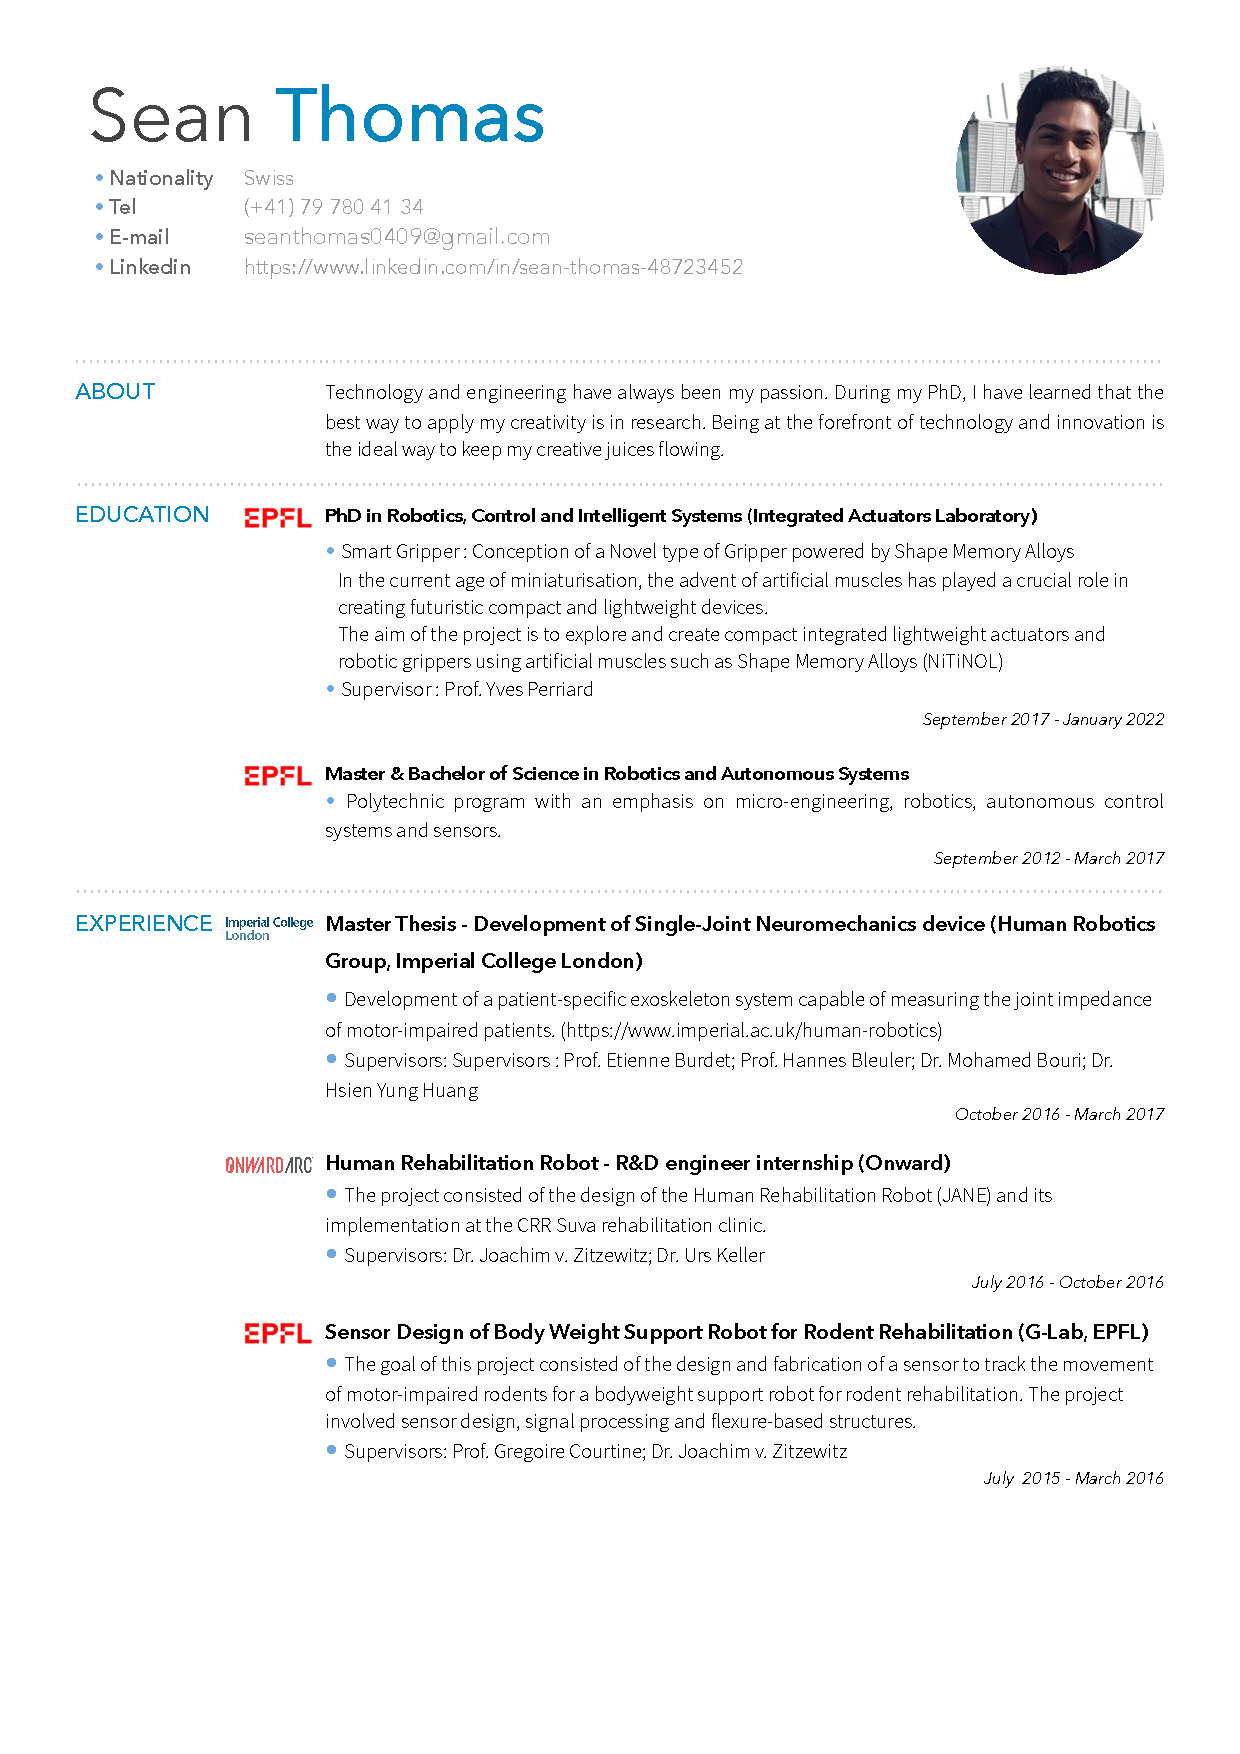
\includepdf[pagecommand=\thispagestyle{addpagenumbersforpdfimports},pages=-]{tail/seanthomas-cv.pdf}
\fi


\end{document}
